\begin{ujnappendix}
\section[附录]{附\qquad 录}
% 以下为附录,把点引线以下的文字替换成你的就好
% ·································································································
    \subsection*{附录A 计算机的层次模型}
        \begin{figure}[htbp]
            \centering
            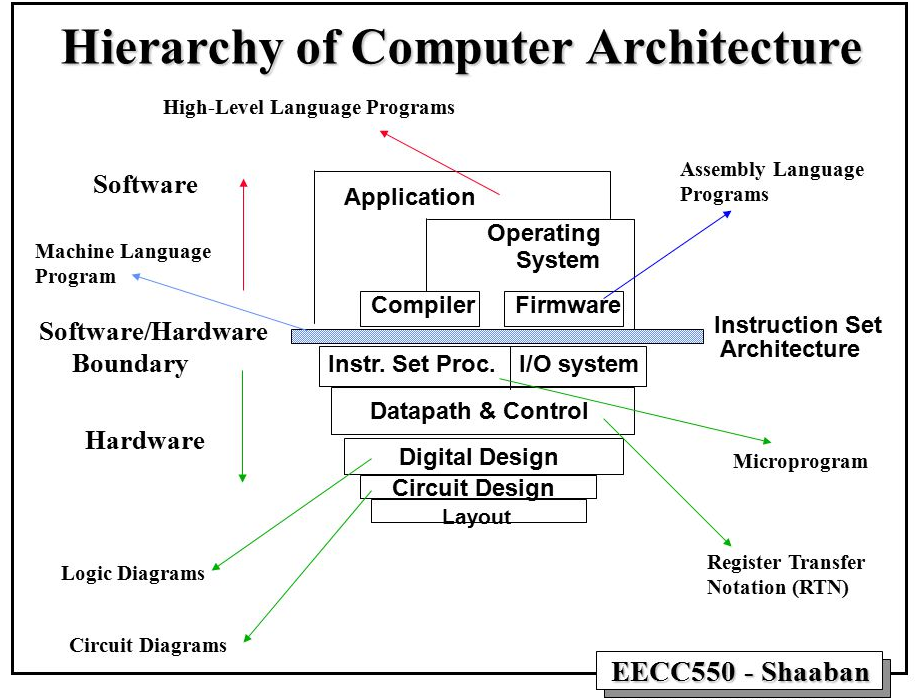
\includegraphics[width=0.8\textwidth]{figures/computer-arch.png}
            \caption{计算机的层次模型}
            \label{fig:computer-arch}
        \end{figure}
    \subsection*{附录B RV32I Base Integer Instruction Set}
% ·································································································
\end{ujnappendix}
